%%
%% licence       kaneton licence
%%
%% project       kaneton
%%
%% file          /home/mycure/kaneton/view/exams/arch-mips/2006/arch-mips-2006.tex
%%
%% created       julien quintard   [fri dec  2 22:25:51 2005]
%% updated       julien quintard   [sat dec  3 22:19:42 2005]
%%

%
% template
%

%%
%% licence       kaneton licence
%%
%% project       kaneton
%%
%% file          /home/mycure/kaneton/view/templates/exam.tex
%%
%% created       julien quintard   [fri dec  2 22:20:57 2005]
%% updated       julien quintard   [mon feb 20 23:01:50 2006]
%%

%
% compile mode
%

%
% ---------- header -----------------------------------------------------------
%
% project       kaneton
%
% license       kaneton
%
% file          /home/mycure/kane...w/talk/presentations/kaneton/kaneton.tex
%
% created       julien quintard   [mon may 14 21:02:29 2007]
% updated       julien quintard   [sun feb  6 20:50:37 2011]
%

%
% ---------- setup ------------------------------------------------------------
%

%
% path
%

\def\path{../../..}

%
% template
%

%
% ---------- header -----------------------------------------------------------
%
% project       kaneton
%
% license       kaneton
%
% file          /home/mycure/kaneton/view/template/talk.tex
%
% created       julien quintard   [wed may 16 18:17:37 2007]
% updated       julien quintard   [fri may 23 19:28:10 2008]
%

%
% ---------- class ------------------------------------------------------------
%

\documentclass[8pt]{beamer}

%
% ---------- common -----------------------------------------------------------
%

\input{\path/package/opk/presentation.tex}


%
% title
%

\title{kaneton}

%
% document
%

\begin{document}

%
% title frame
%

\begin{frame}
  \titlepage
\end{frame}

%
% outline frame
%

\begin{frame}
  \frametitle{Outline}

  \tableofcontents
\end{frame}

%
% ---------- text -------------------------------------------------------------
%


%
% overview
%

\section{Overview}

% 1)

\begin{frame}
  \frametitle{Introduction}

  \term{kaneton} is an educational project intended for students to undertake
  in order to learn about operating system internals.
\end{frame}

% 2)

\begin{frame}
  \frametitle{History}

  \begin{itemize}
    \item[2004]
      \name{Julien Quintard} and \name{Jean-Pascal Billaud} decide
      to introduce an optional low-level programming course to first-year
      enginnering students, now known as \name{kastor};
    \item[2004]
      The course having been well received, \name{SRS - Syst\`emes, R\'eseaux,
      S\'ecurit\'e} students ask them to give such an introductory course the
      same year.
    \item[2005]
      The authorization is given to them to teach a kernel development course
      to \name{SRS} students, from January to October. They therefore decide
      to provide students with the design of a microkernel and let the students
      develop it from scratch, their way. \name{kaneton} is born.
    \item[2006]
      After \name{Jean-Pascal Billaud} fled to \name{VMWare}, \name{Julien
      Quintard} started developing a reference implementation and gave
      students this year a skeleton they had to complete. In addition,
      \name{Cedric Aubouy} and \name{Renaud Lienhart} joined the teaching
      team this year.

      \-

      Besides, the \name{LSE - Laboratoire Syst\`eme EPITA} joined the project
      by putting two students on the development of the \name{kaneton}
      research implementation. \name{Matthieu Bucchianeri} and \name{Renaud
      Voltz} thus joined the project.
  \end{itemize}
\end{frame}


% 3)

\begin{frame}
  \frametitle{History}

  \begin{itemize}
    \item[2007]
      This year, \name{Matthieu Bucchianeri} and \name{Renaud Voltz} took
      over the project for a year by lecturing the course and managing the
      project.

      \-

      \name{Julian Pidancet} and \name{Pierre Duteil} joined the project
      as part of the \name{LSE} but \name{Pierre Duteil} had to leave the
      project. Therefore, \name{Elie Bleton}, who was working at the
      \name{LRDE} before, joined the project.
    \item[2008]
      \name{Julian Pidancet} and \name{Elie Bleton} took over this year
      while \name{Laurent Lec} and \name{Nicolas Grandemange} joined as part
      of the \name{LSE}.

      \-

      At the end of this year, after problems with some students as well as
      conflicts with the \name{LSE}, \name{kaneton} maintainers decided not
      to work with the laboratory anymore.
    \item[2009]
      \name{EPITA} alumni were contacted and joined the educational project
      including \name{Francois Goudal}, \name{Benoit Marcot},
      \name{Enguerrand Raymond}, \name{Jean Guyader} but also
      \name{Fabien Le-Mentec}, an \name{EPITECH} alumnus.
  \end{itemize}
\end{frame}

% 4)

\begin{frame}
  \frametitle{Model}

  The project consists for students to fill in some missing parts of the
  kernel.

  \-

  However, note that, unlike \name{Tiger}, the missing parts will never
  be two lines long.

  \-

  Indeed, in \name{kaneton}, students are asked to implement a feature, say,
  providing memory management. Thus, students are free, in a certain way,
  to implement such a feature as they wish.

  \-

  Since the testing usually consists in verifying that the kernel is able
  to provide the functionality, students should be, most of the time, able
  to implement whatever algorithms \etc{} they wish.
\end{frame}

% 5)

\begin{frame}
  \frametitle{People}

  Let's present the people working on the educational project from where they
  studied to what they are now doing:

  \begin{itemize}
    \item
      \name{Francois Goudal};
    \item
      \name{Benoit Marcot};
    \item
      \name{Jean Guyader};
    \item
      \name{Baptiste Afsa}
    \item
      \name{Louis Vatier}; and
    \item
      \name{Julien Quintard}.
  \end{itemize}
\end{frame}

% 6)

\begin{frame}
  \frametitle{Project}

  \name{kaneton} is an important assignment of the \name{SRS}/\name{GISTR}
  curriculum and, as such, must be taken seriously.

  \-

  Especially, in the last years, \name{EPITA} decided to reduce the duration
  of the project to \term{three} months.

  \-

  As such, the other assignments imposed by the specializations in this
  period have been reduced so that students can focus on \name{kaneton}.
\end{frame}

%
% design
%

\section{Design}

% 1)

\begin{frame}
  \frametitle{Overview}

  The kaneton kernel is very different from the kernels you might be
  familiar with, especially the well-known \name{Windows}, \name{Linux},
  \name{BSD} and so forth.
\end{frame}

% 2)

\begin{frame}
  \frametitle{Microkernel}

  First, kaneton is a microkernel, making it modular from the design
  perspective as well as providing properties such as security.
\end{frame}

% 3)

\begin{frame}
  \frametitle{Distributed Computing}

  kaneton has been designed from the ground up for providing the operarting
  system advanced distributed computing features.
\end{frame}

% 4)

\begin{frame}
  \frametitle{Portability}

  kaneton has been designed with portability in mind, especially through
  a specific portability system that perfectly fits the kernel design.
\end{frame}

% 5)

\begin{frame}
  \frametitle{Organisation}

  Besides being a microkernel, kaneton is well organised in the inside,
  splitting functionalites into objects and managers.
\end{frame}

%
% stages
%

\section{Stages}

% 1)

\begin{frame}
  \frametitle{k0}

  The first project, named \term{k0}, consists for students to learn
  about low-level programming.

  \-

  This project comes with a lecture regarding the boot system as well
  as a practical session.

  \-

  \name{Francois Goudal} will be in charge of this stage which will last for
  a week.
\end{frame}

% 2)

\begin{frame}
  \frametitle{k1}

  \term{k1} consists for students to provide the kaneton microkernel the
  capacity to handle events.

  \-

  During this stage, a lecture on general kernel principles and a lecture on
  interrupts will be taught.

  \-

  \name{Julien Quintard} will be in charge of this stage which will last
  for a single week.

  \-

  Note that, starting with \name{k1}, the student snapshot will be used which
  provide students a development environment, making kernel development easier.
\end{frame}

% 3)

\begin{frame}
  \frametitle{k2}

  \term{k2} consists for students to provide the kaneton microkernel a
  memory management unit so that applications as well as the kernel itself
  can reserve, share \etc{} memory.

  \-

  During this stage, a lecture on portability as well as lectures on
  memory management will be taught.

  \-

  \name{Francois Goudal} will be in charge of this stage which will last
  for three weeks.
\end{frame}

% 4)

\begin{frame}
  \frametitle{k3}

  In \term{k3}, students will have to provide kaneton with execution contexts
  such that the kernel can execute multiple threads at the \textit{same} time.

  \-

  Lectures, during this stage, will discuss topics such as interrupts,
  concurrency, multi-processing, scheduling \etc{}

  \-

  \name{Benoit Marcot} will be in charge of this stage which will last for
  three weeks.
\end{frame}

% 5)

\begin{frame}
  \frametitle{Evaluation}

  For every stage, students will have the possibility to test their
  implementation by running, a limited number of times, the test suite used
  for evaluating their work.

  \-

  Besides, at the end of each stage, after submission, the kaneton test system
  will run the test suite and issue a mark according to the test results.

  \-

  Additionally, an exam will take place at the end of the semester to make
  sure that the notions tackled throughout the course are well understood
  by every student.
\end{frame}

%
% tools
%

\section{Tools}

% 1)

\begin{frame}
  \frametitle{Overview}

  The kaneton educational project relies on tools, sometimes developed
  internally.
\end{frame}

% 2)

\begin{frame}
  \frametitle{Web Site}

  The web site contains the documentation including design papers,
  the assignments \etc{} but also hosts the wiki which should be
  the starting point for every student seeking information.

  \-

  Noteworthy is that the wiki contains courses regarding the
  inline assembly, linking, pre-processing and so on. Students
  are invited to read them all as they will come handy when
  developing the kaneton stages.

  \-

  \name{Julien Quintard} should be contacted for requests regarding the
  web site and wiki.
\end{frame}

% 3)

\begin{frame}
  \frametitle{Snapshot}

  The student snapshot has been automatically generated from the current
  kaneton implementation.

  \-

  \name{Francois Goudal} is in charge of this process, hence should be
  contacted if you believe there is a mistake.
\end{frame}

% 4)

\begin{frame}
  \frametitle{Cheat}

  Every student's kaneton implementation will be tested to make sure that
  students did not cheat by relying on implementations by previous or
  current students.

  \-

  \name{Julien Quintard} is in charge of this tool.
\end{frame}

% 5)

\begin{frame}
  \frametitle{Test}

  Students' implementation will be tested in a real environment by applying
  a complete test suite; hence, validating the implementation's behaviour.

  \-

  \name{Jean Guyader} is responsible of this tool and should be contacted
  if necessary.
\end{frame}

%
% information
%

\section{Information}

% 1)

\begin{frame}
  \frametitle{Support}

  \begin{enumerate}
    \item
      \term{Website}

      \-

      You will find on \location{http://kaneton.opaak.org} documents regarding
      the project from the design to the implementation;
    \item
      \term{Wiki}

      \-

      The wiki \location{http://wiki.opaak.org} is the best way to get
      technical information as well as to help other students by adding
      and/or improving pages' contents;
    \item
      \term{Mailing-List}

      \-

      The kaneton educational students mailing-list
      \location{students@kaneton.opaak.org} will be used by teachers as
      an official means for communicating with students.

      \-

      Therefore, every student should subscribe to this mailing-list by sending
      an email to \location{students+subscribe@kaneton.opaak.org}.

      \-

      It is not allowed to post code on the mailing list, or give pointers to
      code in the snapshot that would provide obvious solution to somebody's
      question.
  \end{enumerate}
\end{frame}

% 2)

\begin{frame}
  \frametitle{Groups}

  Except for \name{k0} which is an individual project, the other projects
  from \name{k1} to \name{k3} are done in groups of \term{two} students.

  \-

  Every group is expected to send an email to
  \location{admin@opaak.org}.

  \-

  Note that we will use students' \name{EPITA} email addresses. As such,
  make sure that you check this email box.
\end{frame}

% 3)

\begin{frame}
  \frametitle{Reliance}

  As for \name{Tiger}, every stage depends on the previous one, except
  for \name{k0}.

  \-

  As such, test suites from the previous stages will also be used for both
  testing and marking.

  \-

  Students should therefore make sure to use their test permissions for making
  sure to fix the bugs of previous stages so that such bugs do not impact
  on the current stage results, hence mark.
\end{frame}

% 4)

\begin{frame}
  \frametitle{Machine}

  This year, the machine used by the kaneton educational project will consists
  of the \term{IBM-PC} platform coupled with the \term{IA-32} microprocessor
  architecture \ie{} the most common hardware system on the market.

  \-

  Although it is always best to test your implementation on a real machine,
  it takes time to reboot a real computer. You should therefore use an
  emulator such a \name{QEMU} or \name{Bochs} as they will enable you to
  test your kernel very quickly but they will also let you develop on
  a non-\name{IBM-PC}/\name{IA-32} machine such as a \name{Mac} for example.
\end{frame}

%
% conclusion
%

\section{Conclusion}

% 1)

\begin{frame}
  \frametitle{Concepts}

  Throughout the project, you will learn so many things from terminology,
  to how a computer boots, how the kernel controls the hardware and how it
  provides abstractions as basic as execution contexts.

  \-

  At the end of the project, you will definitely know that nothing is magic
  but purely logic and often actually very simple.
\end{frame}

% 2)

\begin{frame}
  \frametitle{Implementation}

  Although, starting the project by learning how to make a computer execute
  your code, you will end up, after three months, with a running kernel
  and operating system capable of executing programs, the whole on real
  hardware like the machine you have at home.
\end{frame}

% 3)

\begin{frame}
  \frametitle{Changes}

  Over the years, the project has greatly evolved, from a no-implementation
  project, to a reference-based project.

  \-

  However, being a project developed by volunteers willing to dedicate some
  time so that other students can learn, many things are missing and/or
  can be improved including the lectures but also the project implementation.

  \-

  In conclusion, keep in mind that the project exists only because of people
  willing to transfer their knowledge and please respect their effort.
\end{frame}

% 4)

\begin{frame}
  \frametitle{Fun}

  But most of all, kaneton should be about learning through fun!
\end{frame}

% 5)

\begin{frame}
  \frametitle{Reminder}

  Remember to perform the following tasks:

  \begin{itemize}
    \item
      Send an email to \location{admin@opaak.org} regarding the composition
      of your group, before \textbf{Wednesday 16th 2pm} or you will be put
      in a group by force;
    \item
      Subscribe to the students mailing-list
      \location{students@kaneton.opaak.org} by sending an email to
      \location{students+subscribe@kaneton.opaak.org};
    \item
      Watch closely the \name{Wiki} at \location{http://wiki.opaak.org} by
      subscribing the \name{RSS} feed for example;
    \item
      We advise SRS/GISTR lab roots to set up a \name{Xen}-based environment
      as testing on emulators only will become difficult over time;
    \item
      Students must have a ``rack'' containing a \name{POSIX}-compilant
      operating system for the \name{k0} practical session.
  \end{itemize}
\end{frame}

\end{document}


%
% class
%

\documentclass[10pt,a4wide]{article}

%
% packages
%

\usepackage[english]{babel}
\usepackage[T1]{fontenc}
\usepackage{a4wide}
\usepackage{graphicx}
\usepackage{fancyheadings}
\usepackage{multicol}
\usepackage{indentfirst}
\usepackage{color}
\usepackage{ifthen}
\usepackage{comment}
\usepackage{verbatim}
\usepackage{aeguill}

\pagestyle{fancy}

\setlength{\footrulewidth}{0.3pt}
\setlength{\parindent}{0.3cm}
\setlength{\parskip}{2ex plus 0.5ex minus 0.2ex}

%
% correction environment
%

\newenvironment{correction}%
   {
     \ifthenelse
	 {
	   \equal{\kaneton-latex}{subject}
	 }
	 {
	   \comment
	 }
	 {
	   \textbf{\color{red}{ ----- correction}}
	 }
   }%
   {
     \ifthenelse
	 {
	   \equal{\kaneton-latex}{subject}
	 }
	 {
	   \endcomment
	 }
	 {
	   \textbf{\color{red}{ ----- /correction}}
	 }
   }

%
% header
%

\rfoot{\scriptsize{Exam}}

\date{\scriptsize{\today}}


%
% correction mode
%

\newboolean{cmode}
\setboolean{cmode}{false}

%
% header
%

\lhead{\scriptsize{2006}}

%
% title
%

\title{Examen d'Architecture MIPS}

%
% authors
%

\author{\small{Julien Quintard}}

%
% document
%

\begin{document}

%
% title
%

\maketitle

%
% --------- information -------------------------------------------------------
%

\begin{center}

\textbf{Documents Autoris\'es}

\textbf{Dur\'ee 3 heures}

\scriptsize{Une copie bien pr\'esent\'ee avec des sch\'emas propres et
	    lisibles sera toujours mieux not\'ee qu'une autre.}
\end{center}

%
% --------- text --------------------------------------------------------------
%

On consid\`ere la fonction \textbf{strncpy} d\'ecrite ci-dessous
en langage C.

\begin{verbatim}
char*           strncpy(char* dst, const char* src, unsigned int size)
{
  int           i;

  for (i = 0; i < size && src[i]; i++)
    dst[i] = src[i];
  dst[i] = 0;

  return (dst);
}
\end{verbatim}

Ce code f\^ut ensuite compil\'e pour une r\'ealisation \textbf{non pipeline}
du processeur MIPS. Le code assembleur produit est le suivant:

\begin{verbatim}
         Lw R5, 0(R29)
         Lw R6, 4(R29)
         Lw R7, 8(R29)

         Add R2, R5, R0

         Add R16, R6, R7

Loop:    Lb R10, 0(R6)
         Beq R10, R0, EndLoop

         Sb R10, 0(R5)

         Addiu R5, R5, 1
         Addiu R6, R6, 1

         Bne R6, R16, Loop

EndLoop: Sb R0, 0(R5)

         Jr R31
\end{verbatim}

%
% fonctionnement
%

\section{Fonctionnement}

Modifier ce code de telle mani\`ere qu'il soit ex\'ecutable par le processeur
pipeline 5 \'etages MIPS etudi\'e en cours.

Faites le lien entre les registres et le programme C. Notamment,
nous attendrons l'identification des variables \textit{dst}, \textit{src}
et \textit{size}.

Vous expliquerez ensuite l'algorithme utilis\'e en assembleur, c'est-\`a-dire
les diff\'erentes \'etapes assembleur.

%\verbatimboxed{Makefile}

\begin{correction}

  Il faut ajouter les \textit{delay slots} apr\`es chaque branchement.

  \begin{verbatim}
           Lw R5, 0(R29)
           Lw R6, 4(R29)
           Lw R7, 8(R29)

           Add R2, R5, R0

           Add R16, R6, R7

  Loop:    Lb R10, 0(R6)
           Beq R10, R0, EndLoop
           Nop

           Sb R10, 0(R5)

           Addiu R5, R5, 1
           Addiu R6, R6, 1

           Bne R6, R16, Loop
           Nop

  EndLoop: Sb R0, 0(R5)

           Jr R31
           Nop
  \end{verbatim}

  Voici les liens entre le code assembleur et le code C:

  \begin{itemize}
    \item
      \textit{R5}: dst.
    \item
      \textit{R6}: src.
    \item
      \textit{R7}: size.
    \item
      \textit{R16}: src + size.
    \item
      \textit{R10}: src[i].
  \end{itemize}

  L'algorithme utilis\'e est le suivant:

  \begin{enumerate}
    \item
      R\'ecup\'eration des arguments de la fonction: \textit{R5}, \textit{R6},
      \textit{R7}.
    \item
      Affectation \`a la valeur de retour la valeur du pointeur \textit{dst}:
      \textit{R2}.
    \item
      Calcul de l'adresse de fin de la cha\^ine de caract\`eres source:
      \textit{R16}.
    \item
      Tant que le pointeur de la chaine source est diff\'erent de \textit{R16}.
    \item
      Lecture du caract\`ere courant: \textit{R10}.
    \item
      Si le caract\`ere courant est le caract\`ere z\'ero, sortir de la boucle.
    \item
      \'Ecriture du caract\`ere dans la cha\^ine destination: \textit{R5}.
    \item
      Incr\'ementer les pointeurs des cha\^ines source et destination:
      \textit{R5}, \textit{R6}.
    \item
      Si on est arriv\'e \`a la fin de la boucle, en sortir.
    \item
      \'Ecriture du caract\`ere z\'ero dans la cha\^ine destination:
      \textit{R5}.
    \item
      Retour du au programme appelant.
  \end{enumerate}

\end{correction}

%
% analyse simplifiee
%

\section{Analyse Simplif\'ee}

On consid\`ere le processeur pipeline MIPS \'etudi\'e en cours, compos\'e
de cinq \'etages.

Analyser l'ex\'ecution d'une it\'eration de boucle \`a l'aide d'un
sch\'ema simplifi\'e.

Calculer ensuite le nombre moyen de cycles n\'ecessaires \`a
l'ex\'ecution d'une it\'eration de la boucle. Calculer le CPI utile
(en consid\'erant qu'un NOP n'est pas une instruction utile).

\begin{correction}

  \begin{center}
    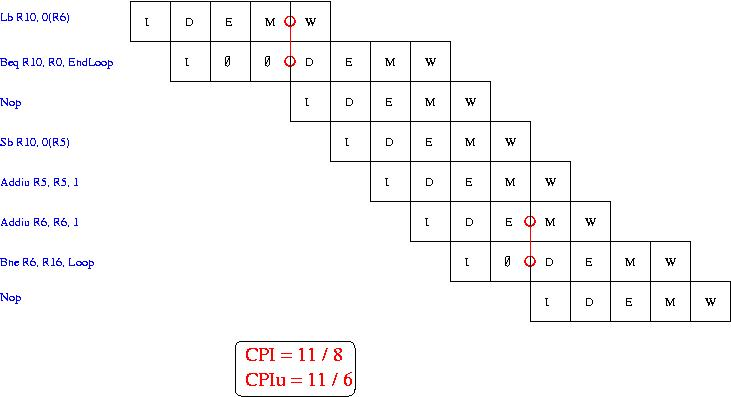
\includegraphics[scale=0.7]{figures/correction-analyse-simplifiee.jpg}
  \end{center}

\end{correction}

%
% reordonnancement
%

\section{R\'eordonnancement}

R\'eordonner le code assembleur de la boucle de mani\`ere \`a \'eviter
au maximum les cycles de gel et les cycles perdus dans les \textit{delay slots}.

Combien de cycles sont d\'esormais n\'ecessaires \`a l'ex\'ecution d'une
it\'eration?

\begin{correction}

  \begin{verbatim}
  Loop:    Lb R10, 0(R6)

           Addiu R5, R5, 1
           Addiu R6, R6, 1

           Beq R10, R0, EndLoop
           Nop

           Bne R6, R16, Loop
           Sb R10, -1(R5)
  \end{verbatim}

  Il faut d\'esormais \textbf{7} cycles pour l'ex\'ecution d'une it\'eration.
  Il ne reste plus de cycles de gel, n\'eanmoins il subsiste un
  \textit{delay slot} non utilis\'e.

\end{correction}

%
% analyse detaillee
%

\section{Analyse Detaill\'ee}

Donner un sch\'ema detaill\'e de l'ex\'ecution de la s\'equence d'instructions
suivante dans le pipeline classique MIPS 5 \'etages:

\begin{verbatim}
Lw R3, 0(R5)
Add R5, R1, R3
\end{verbatim}

\begin{correction}

  \begin{center}
    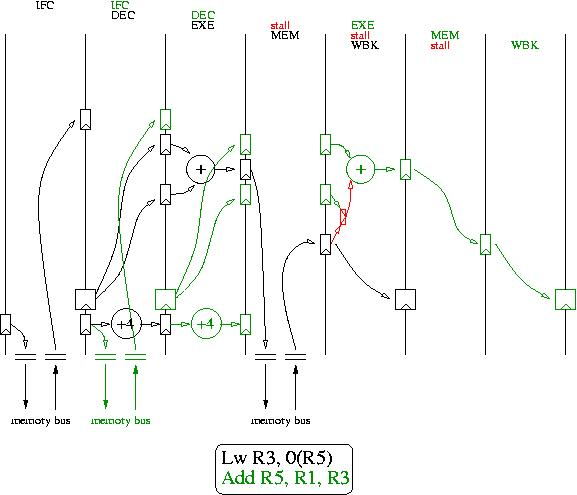
\includegraphics[scale=0.7]{figures/correction-analyse-detaillee.jpg}
  \end{center}

\end{correction}

%
% pipeline
%

\section{Pipeline}

On consid\`ere le processeur pipeline P construit autour d'un pipeline
\`a 7 \'etages.

En effet, l'\'etage IFC a \'et\'e d\'ecoup\'e: l'acc\`es m\'emoire commence
en IFC-1 et se termine en IFC-2.

De plus l'\'etage DEC a \'egalement \'et\'e d\'ecoup\'e. L'\'etage
DEC-1 d\'ecode et extrait les op\'erandes alors que l\'etage DEC-2 calcule
l'adresse de l'instruction suivante incluant bien entendu la comparaison
des op\'erandes dans le cas d'un branchement conditionnel.

\begin{center}
  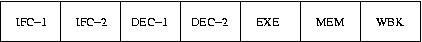
\includegraphics[scale=0.7]{figures/pipeline.jpg}
\end{center}

Combien de bypasses existent-ils sur ce processeur?

Representer ces bypasses sur un schema simplfi\'e?

Donner un exemple de code mettant en \'evidence chacun de ces bypasses.

\begin{correction}

  Il y a exactement \textbf{5} bypasses.

  \begin{center}
    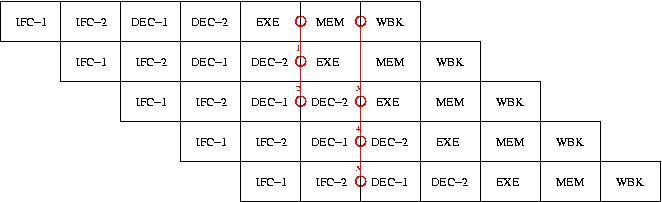
\includegraphics[scale=0.7]{figures/correction-pipeline.jpg}
  \end{center}

  \begin{enumerate}
    \item
      \begin{verbatim}
	Add R3, R2, R1
	Add R5, R4, R3
      \end{verbatim}
    \item
      \begin{verbatim}
	Add R3, R2, R1
	Nop
	Beq R3, R0, Loop
      \end{verbatim}
    \item
      \begin{verbatim}
	Lw R3, 0(R5)
	Nop
	Add R5, R4, R3
      \end{verbatim}
    \item
      \begin{verbatim}
	Lw R3, 0(R5)
	Nop
	Nop
	Beq R3, R0, Loop
      \end{verbatim}
    \item
      \begin{verbatim}
	Lw R3, 0(R5)
	Nop
	Nop
	Nop
	Beq R3, R0, Loop
      \end{verbatim}
  \end{enumerate}

  \`A noter que la s\'equence:

  \begin{verbatim}
    Add R3, R2, R1
    Nop
    Nop
    Beq R3, R0, Loop  
  \end{verbatim}

  utilise le bypass num\'ero \textbf{4}.

\end{correction}

%
% optimisations
%

\section{Optimisations}

Modifier le code assembleur originel de la fonction \textbf{strncpy} de
mani\`ere \`a ce qu'il soit ex\'ecutable sur le processeur P.

Puis effectuer les optimisations suivantes sur la boucle du code
pr\'ec\'edemment obtenu:

\begin{itemize}
  \item
    R\'eordonnancement.
  \item
    Loop Unrolling.
\end{itemize}

Pour chacune de ces optimisations, vous devrez calculer le nombre de cycles
n\'ecessaire au traitement d'un \'el\'ement de la cha\^ine.

\begin{correction}

  Voici le code modifi\'e de mani\`ere \`a \^etre ex\'ecutable sur le
  processeur P.

  Il faut tout simplement prendre en compte les \textit{delay slots}.

  \begin{verbatim}
           Lw R5, 0(R29)
           Lw R6, 4(R29)
           Lw R7, 8(R29)

           Add R2, R5, R0

           Add R16, R6, R7

  Loop:    Lb R10, 0(R6)
           Beq R10, R0, EndLoop
           Nop
           Nop

           Sb R10, 0(R5)

           Addiu R5, R5, 1
           Addiu R6, R6, 1

           Bne R6, R16, Loop
           Nop
           Nop

  EndLoop: Sb R0, 0(R5)

           Jr R31
           Nop
           Nop
  \end{verbatim}

  \textbf{R\'eordonnancement}

  \begin{verbatim}
  Loop:    Lb R10, 0(R6)

           Addiu R5, R5, 1
           Addiu R6, R6, 1

           Beq R10, R0, EndLoop
           Nop
           Nop

           Bne R6, R16, Loop
           Sb R10, -1(R5)
           Nop
  \end{verbatim}

  \textbf{9} cycles sont n\'ecessaires \`a l'ex\'ecution de cette boucle et
  donc au traitement d'un \'el\'ement.

  \textbf{Loop Unrolling}

  \begin{verbatim}
  Loop:    Lb R10, 0(R6)
           Lb R11, 1(R6)

           Addiu R5, R5, 2

           Beq R10, R0, EndLoop
           Addiu R6, R6, 2
           Nop

           Bne R6, R16, Loop
           Sb R10, -2(R5)
	   Sb R11, -1(R5)
  \end{verbatim}

  \textbf{9} cycles sont n\'ecessaires \`a l'ex\'ecution de cette boucle.
  N\'eanmoins, le nombre de \textit{delay slots} a nettement diminu\'e de
  3 \`a 1.

  \'Etant donn\'e que deux caract\`eres de la cha\^ne sont trait\'es tous
  les \textbf{9} cycles, un caract\`ere est en moyenne trait\'e tous les
  \textbf{4.5} cycles.

\end{correction}

\end{document}
